\section{Risk Assessment for Investors}


\subsection{Introduction}

Following the goal set by the Paris Climate Agreement to keep the global temperature increase under 2 degrees by 2100,  it has been estimated that achieving this goal will require approximately 3\% of global GDP in the year 2100 \cite{schleussner2016science, tol2022costs}. The energy sector is responsible for 84\% of CO$_2$ emissions - meaning there is a requirement for vast levels of investment in carbon-free energy. Among these alternatives, Fusion energy stands out as a  zero-emission energy source, since it overcomes the drawbacks faced by wind and solar of requiring efficient energy storage and questions around energy security. 

However, fusion energy faces a number of socio-economic challenges that need to be overcome. Addressing these challenges is important to ensure sufficient implementation, consequently having a tangible impact on meeting the Paris Climate Agreement targets. These risks include the financial uncertainty faced by investors, supply line limitations, a public opinion tarnished by nuclear fission accidents, and safety considerations unique to fusion reactors. These factors are discussed in this review and applied to the specific case of magnetic mirror MIF, with the goal of helping inform strategies for risk mitigation and management.


\subsection{Financial risks}

This section will present the financial risks associated with nuclear fusion, and the impact this has on investment in the sector. Issues of return on investment timeframe, policy and technological uncertainties, and supply chain challenges are discussed. 

\subsubsection{Fusion’s appeal to investors}


The aim of this section is to present the challenges and uncertainties investors are faced with when considering nuclear fusion and compare these against the possible return an investor may expect. According to Jevons,  the value of an investment is determined by its marginal contribution to the investor’s objective system (i.e. the additional value it adds to their specific investment goal or strategy) \cite{jevons1879theory}. Thus the details of the investor’s objective system and decision field are necessary to evaluate risk. In this case, a reasonable decision field would consider the technical and financial properties of fusion power, uncertainties associated with fusion, and macroscopic market conditions. 

\subsubsection{Uncertainties}

Power-generation technologies are, by their nature, long-term investments. For fusion, this fact is especially true as many of the enabling technologies are yet to be developed, and in most cases, engineering designs for a commercial plant are years away. Without considering any other factors, the long timescale alone presents significant uncertainty for the investor. 

This review categorizes uncertainties into three inter-dependent groups: those associated with the extended timeframe, technological considerations, and macroscopic factors. This classification is by no means exhaustive - by definition, an identification of uncertainties cannot be.

\subsubsubsection{Uncertainties associated with the long development and implementation timeframe:}
\begin{itemize}
\item Investors may not see a monetary ROI within their lifetime for some concepts.
 \item Some results reached during the program — e.g. on the properties of materials — may be of no use, and hence produce no royalty income, until the full completion of the program.
 \item Changes in the copyright laws cannot be ruled out.
 \item The duration of patents under present laws appears insufficient.
 \item Technology may become outdated by the time of implementation.
 \item Patents referring to incremental improvements may supersede patents referring to the original development of fusion reactors.
\end{itemize}


\subsubsubsection{Uncertainties ascribed to technological considerations:}
\begin{itemize}
\item Regional construction capacity projections of nuclear fusion.
 \item The capacity utilization ratio of options in energy/environment technologies.
 \item Load-following capability.
 \item High capital costs of emerging technologies.
 \item Uncertainty of payoff from R\&D investments - not all R\&D outputs will be of benefit to fusion or secondary applications.
 \item The visibility of the results to investors and the general public.
 \item The need to set financial limits on R\&D expenditure.
 \item Energy storage technologies.
 \item Resource extraction efficiency (e.g. lithium, deuterium, beryllium).
 \item Laser efficiency for IFE concepts.
 \item Cost, scaling, and large-scale manufacturing of new HTS magnets using, e.g. REBCO tape.
\end{itemize}
 

\subsubsubsection{Uncertainties in macroscopic factors:}
\begin{itemize}
\item Utility discount rates.
 \item Energy demand scenarios.
 \item CO$_2$ target in 2100.
 \item Adjustments in environmental policies.
 \item Prices of emission certificates.
 \item Changes in ecological awareness.
 \item Energy security concerns associated with geopolitical factors.
 \item Public perception of fusion.
 \item The structure of the energy market - fractional contribution of fossil fuels, renewables, and nuclear fission.
 \item Price of fossil fuels.
 \item Changes in perception of impact investments.
\end{itemize}
 

\subsection{Addressing the Economic Uncertainties of Fusion}

\subsubsection{Economic concerns}

The most obvious objective for an investor is to make a financial return on their investment (ROI). Due to the uncertainties outlined above, it would seem that from a financial perspective, fusion is not the most attractive choice \cite{prades2008lay}. When a group of investors with some, but still limited knowledge of fusion, held a discourse as part of Lopez et al.’s study on the lay perception of investments in fusion, the outcome was that ‘Fusion R\&D was perceived to be very expensive’. Their concerns specifically centered on anxiety about investing in R\&D if the technology does not prove a viable energy source, and the long time frame involved. It was found, however, that the prospect became significantly more acceptable if possible spin-off technologies of the program could be identified, and if visible, understandable milestones were achieved. Furthermore, there is a significant overlap between investors who are likely to invest in fusion, and those who are likely to invest in renewables; investment in fusion cannot inhibit progress on renewable energy sources. It is important, then, that fusion companies seeking investment consider the broader applications of their technology; particularly in the setting of renewable energy. In the case of a MIF mirror concept, there are many technological research paths that could have secondary applications including HTS magnet advancements for medicine, byproducts of lithium extraction for the DT fuel, or advanced sensors and diagnostics.

\subsubsection{The effect of market conditions on the economic viability of fusion}

The commercial competitivity, thus the appeal of investment, of nuclear fusion is heavily impacted by policy decisions. In the scenario that the Paris 2 degree 2100 goal is maintained, and a limit of atmospheric CO$_2$ concentration of 450 ppm is enforced, widespread implementation of wind and solar energy will be required in the first half of this century. High feed-in of these technologies will challenge base-load technology and lead to volatile power prices; in this scenario, fusion becomes an attractive offering \cite{klingelhofer2011financial}. If the power output of a fusion plant is dispatchable and can be varied according to demand (i.e. minimal during times of peak solar output - see ‘solar duck curve’, and maximal during times of reduced renewable performance), fusion plants can operate in reserve markets, where they will be competitive even if their cost of electricity is significantly higher than renewables. In a study of hourly electricity costs in southern California energy prices were below the average of \$36.50/MWh for 70\% of 2018, and negative for $\sim$2\% of the year, but as high as \$999/MWh \cite{EPRI2020}. For an energy market with high renewable penetration, dispatchability is a key factor in competitiveness. This benefit is most easily exploited by pulsed fusion concepts, where it is not necessary for a plasma to be set up and maintained.  The MIF with magnetic mirrors concept presented in this report thus has a unique advantage over e.g. Tokamaks in this regard.

Another consideration is the future contribution of fossil fuels to the energy market. In the near future, it is forecast that for the USA and EU, natural gas will be the dominant source of energy, with China, India, and Africa, having larger contributions of oil and coal \cite{kamani2023long}. As natural gas is by far the most abundant, and cleanest of the fossil fuels, it is forecast that natural gas extraction will far exceed that of coal and oil \cite{klingelhofer2011financial}. It is estimated that at the current rate of consumption, natural gas reserves will last for 100 years. However, as the most convenient gas fields are depleted, as in the production of oil, it becomes necessary to develop resources that are more and more difficult and, hence, more and more expensive to recover, driving up the cost of electricity for base-load power generation \cite{arutyunov2017energy}. This is an inevitability that is agnostic of environmental policy such as the 450 ppm CO$_2$ goal.

If carbon pricing is taken seriously, it could have a considerable impact on the economic appeal of fusion. The prices for CO$_2$ certificates are expected to rise to 110 USD in 2030 - zero emissions technology, such as fusion power will always benefit from tightened environmental policy. Further, unlike, for example, solar energy, there is no ceiling for implementation where fusion becomes uneconomical.  See \ref{enviro} for more details on the impact of environmental policy on the implementation of fusion. It has been found that under diligent environmental policy, fusion could see a ‘maximal’ implementation in terms of share of produced electricity in 2100 (up to 30\%), annual total energy systems cost reduction (1\%), and carbon tax reduction (mitigation rate up to 10\% or a few hundred dollars per tonne of carbon) \cite{tokimatsu2003role}. In this scenario, a present-day design of Tokamak could see wide implementation, with a competitive cost of electricity in the range 70–130 m\$/kWh. Considering the high renewable penetration in a market under these conditions, a pulsed concept like MIF could see further implementation.

A consideration for investors should be the fact that although the development period of fusion seems to be long, the outcome could accompany human development for an indefinitely long time \cite{roncaglia1989research}. Either due to total resource depletion or due to environmental restrictions, eventually, ‘humanity has no sources other than fusion energy’ \cite{arutyunov2017energy}. When viewed through this lens, a return on investment in fusion seems inevitable - the current global energy industry is valued at \$ 6 trillion, according to the International Trade Administration. 

\subsubsection{ROI on climate change}

A final, broader consideration is the indirect return on investment gained from investing in zero-carbon energy. The validity of cost-benefit analysis in the context of long-term climate goals has been in question for some time, with a recent assessment concluding that despite the large uncertainties (such as volatility in carbon price), robust conclusions and policy guidance are able to be found \cite{ekholm2018climatic}. A 2020 paper by Glanemann et al. provides an optimizing cost-benefit analysis of the effect of climate change on global GDP, under various climate sensitivities and mitigation costs and uncertainties \cite{glanemann2020paris}. The study found that the most economically optimal policy pathway is to keep the temperature below 2 degrees C, in agreement with the Paris 2016 goals (see figure \ref{fig:climate_gdp}). Another 2020 cost-benefit analysis by Wei et al. finds that by adhering to a global temperature increase of 1.5 degrees C, the global economy would see 0.46 - 5.24\% GDP gains in 2100, compared with current efforts \cite{wei2020self}. This amounts to a loss of 126.68 - 616.12 trillion dollars.

From a governmental perspective, or indirectly for a private investor, investment in zero-carbon energy could see a significant economic return by the end of the century. Due to the ceiling on implementation of variable output renewable energy sources, this must result in investment into steady state alternatives, such as fusion.

\begin{figure}[h!]
    \centering
    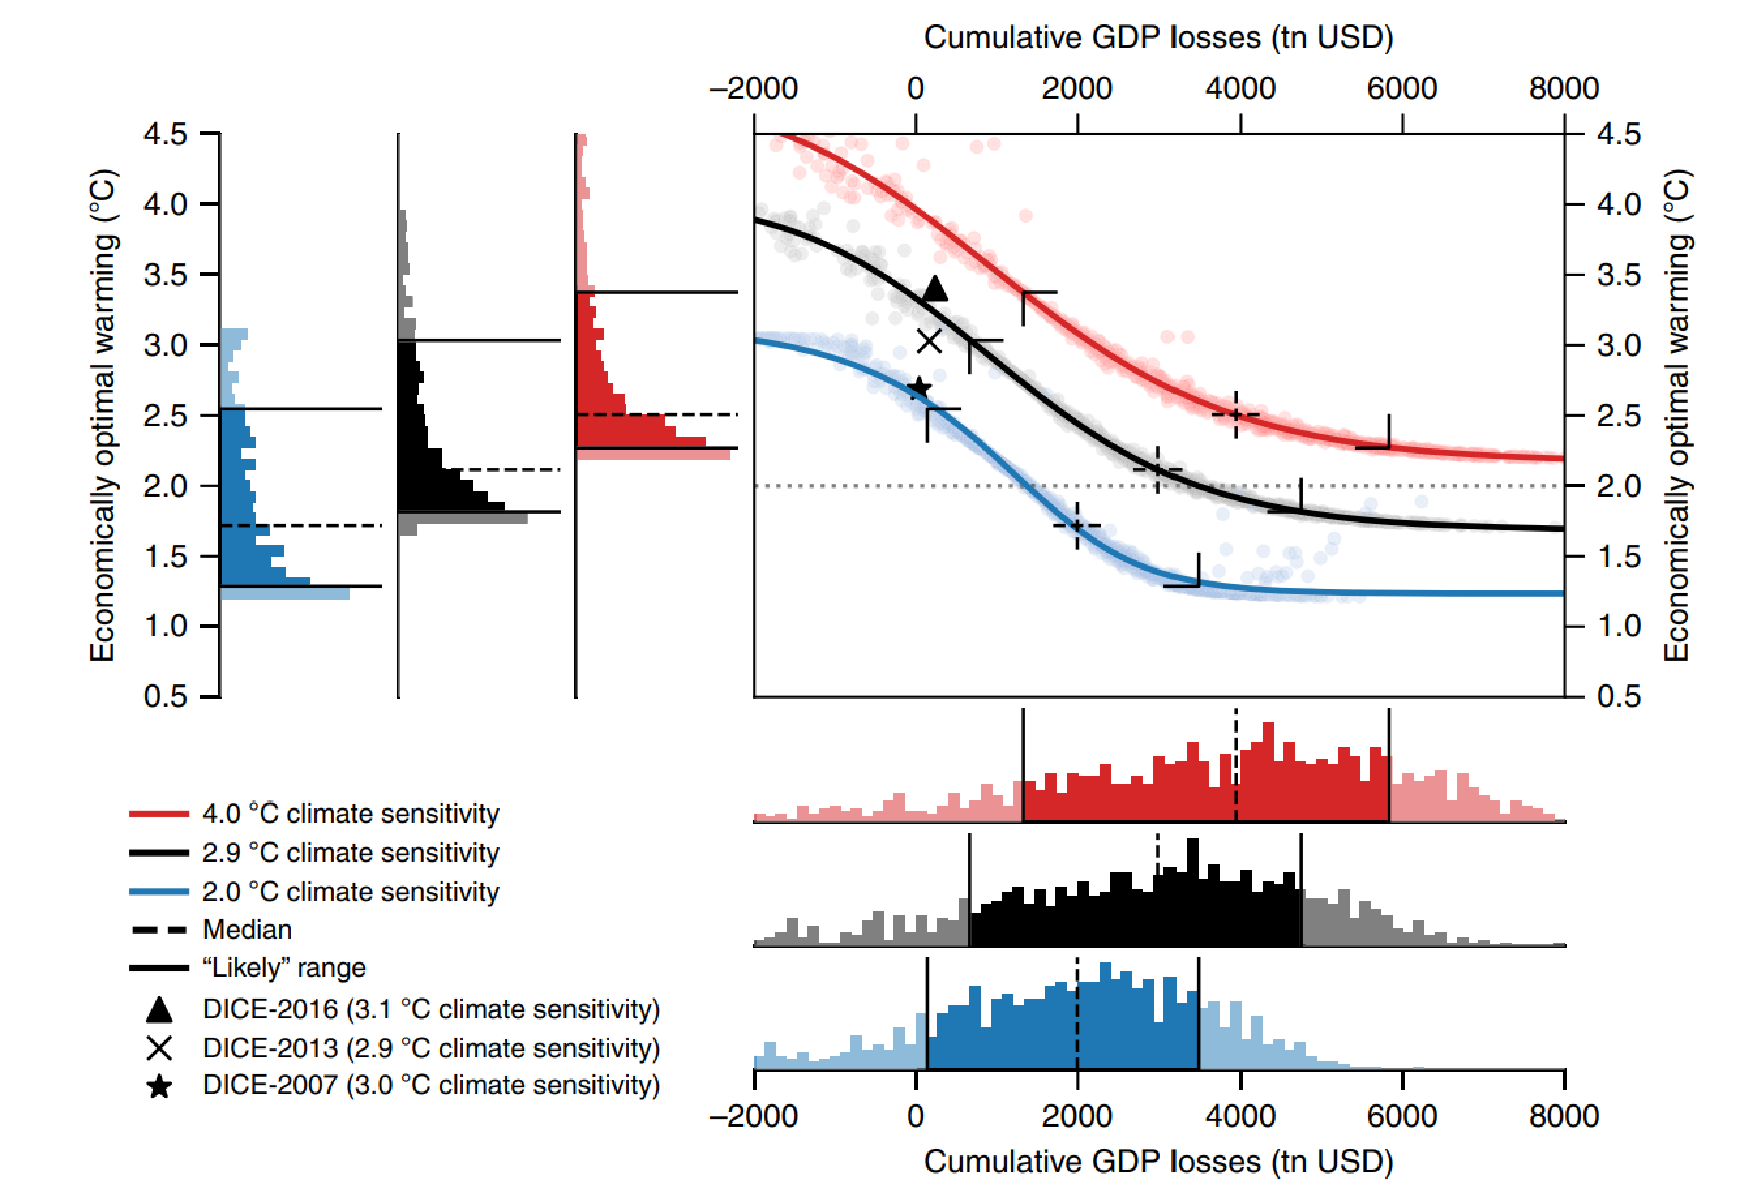
\includegraphics[width =0.65\linewidth]{SubreportFigures/climate_gdp.pdf}
    \caption{Relation between the cumulative GDP losses until 2100 (in 2005 \$US) in the absence of climate policy and the economically optimal warming until the end of the century, given uncertainty in the estimates of the historical impact and uncertainty in the climate sensitivity value. From \cite{glanemann2020paris}. }
    \label{fig:climate_gdp}
\end{figure}




\subsection{Outlook for the investor}

The shifting energy landscape presents a complex outlook for investors in the fusion industry. Energy-economy equilibrium modeling, integrating technological aspects, economic behavior, markets, and policy, can inform the outlook of an investor and identify potential future pathways. The 21st-century energy market, however, is marked by uncertainty and potential major shifts, challenging conventional modeling approaches. In economic models, when multiple technologies produce a homogeneous good, the most cost-effective technology usually prevails. However, this rule often does not hold true in the real world, particularly in the energy sector. Traditional models using constant-elasticity-of-substitution (CES) functions struggle with adapting to market shifts, such as the transition to renewable energy. The IND approach, developed by Landis and Rausch, addresses these discrepancies \cite{landis2017deep}. It treats electricity as a homogeneous good while differentiating technologies based on investment, offering a more accurate reflection of technology market shares and transitions in energy supply. 

For investors in the fusion industry, understanding these dynamics is crucial, especially under strict climate policies. The IND model suggests that as policies increasingly favor low-carbon options, investments in renewable technologies, including fusion, could become more attractive. However, navigating this transition is complex, requiring an understanding of how policy instruments, technological shifts, and market responses interact. Under renewable energy subsidies, the IND model indicates that a complete shift to renewable energy is feasible, a scenario not achievable with standard approaches. This insight is vital for investors, highlighting the evolving nature of the energy market and the potentially significant role of fusion technology in the future energy mix - as policies shift in favor of low-carbon options ‘investments in renewable energy technologies can become increasingly attractive’. The study concludes that in the face of such an uncertain energy landscape, investors need a nuanced understanding of the energy sector's transformation dynamics, especially under strict climate policies.

Most of the considerations thus far have been economic, as that is the primary concern of the private investor. However, for fusion, it has been argued that financial ROI should not be the only metric of profitability \cite{roncaglia1989research}. Notably, fusion has the potential for environmental and ecological benefits, societal benefits from a prosperous startup and research industry, and long-term human development. These factors, alongside the growing issue of energy security, have, to date, primarily only been the concern of governments. Indeed, when considering the Paris climate pledges, and geopolitical motivations, the case for fusion to governments is particularly appealing. 

Historically, private investment has been limited and left to the realm of altruistic or philanthropic high-net-worth individuals \cite{halem2021financing}. However, if fusion is to become a major contributor to global energy supply, it needs significant, widespread private investment, and it is private investors who must consider non pecuniary benefits, alongside the economic case for fusion. So-called ‘impact investing’ could be a primary motivation for private investment in fusion, considering all the potential benefits of fusion development, instead of a purely economic rationale \cite{clarkin2016impact}. In a study by Barber et al., an analysis of the acceptability of returns of an impact investment fund was performed with 3460 investors of limited partner designations across the financial sector \cite{barber2021impact}. The result was that investors were willing to accept a 2.5-3.7 percentage points lower return on an impact investment, than a traditional fund. Thus, even in the scenario of limited economic return on investment, fusion could still find widespread funding as an impact investment.




\subsubsection{Outreach}

This section addresses the challenges and strategies of public outreach in fusion energy investment, focusing on the introduction of nuclear energy to new regions. It emphasizes the importance of considering cultural, political, and historical contexts and local concerns, particularly when nuclear energy is being introduced for the first time. The National Nuclear Laboratory's (NNL) role in educating those involved in the nuclear sector is highlighted, demonstrating the necessity of informed and skilled public engagement. Key factors for successful outreach include addressing safety and security, transparent communication, understanding cultural attitudes towards nuclear energy, building public trust, and balancing the complexity of information presented. This section provides a guide to effective public engagement in the context of fusion energy investment.

In addressing the risks associated with public engagement, it is paramount to consider the underlying context before initiating any outreach program. Caution is advised against assuming that increased engagement will invariably yield beneficial outcomes. This underscores the need for a thoughtful examination of cultural, political, and historical factors, and specific local concerns. This caution is particularly pertinent when introducing nuclear energy to a country for the first time, necessitating a nuanced and context-specific approach \cite{holmes2019developing}.

Effective public management necessitates a well-informed and educated sector adept at navigating public engagement challenges. Recognizing this imperative, the National Nuclear Laboratory (NNL) has taken the initiative to educate individuals involved in or interested in the nuclear sector through a series of enlightening lectures \cite{NNL2020}.

For successful public outreach concerning a magnetic mirror fusion reactor, and more broadly, any nuclear facility, it is crucial to consider several factors based on insights provided by the NNL \cite{holmes2019developing}. Primarily, acknowledging and addressing the safety and security of the nuclear industry is pivotal, emphasizing its contributions to energy security and economic growth. Public engagement should be approached transparently, whether from a neutral or positive standpoint or as a means to counter negative preconceptions.

Understanding the national culture is essential, in determining whether the public is more influenced by factual or emotion-based considerations. Building and sustaining public trust in the nuclear industry and its scientists are imperative, while also recognizing the perceived linkage between civil nuclear power and nuclear weapons. Striking a delicate balance in providing sufficient detail for understanding without overwhelming the audience is crucial, considering the level of familiarity with nuclear matters at both national and local levels.

\subsubsection{Inclusion}

Recognizing the different roles of government, industry, independent experts, and others in the nuclear communications landscape is vital for a coordinated national approach. Utilizing a mix of communication channels, including traditional one-way channels and more interactive two-way channels like face-to-face contact and social media, is recommended. However, it is acknowledged that the latter, while more effective, requires more labor-intensive efforts and can lead to challenging discussions \cite{holmes2019developing}.


\subsection{Safety}

\subsubsection{Fusion}

Despite the diversity in fusion reactor designs, it is possible to identify shared patterns in the principal risks and safety challenges, providing a basis for discussion and analysis.

The use of the D-T reaction in fusion reactors gives rise to several safety challenges that need resolution during the design phase. The primary safety concerns for D-T burning reactors revolve around minimizing and controlling radioactive inventories, specifically tritium and activation products generated through the interaction of fusion reactor materials with high-energy neutrons produced in the fusion reaction.
Notable design issues stemming from these inventories include:
\begin{itemize}
    \item Reduction of radioactive inventories;
\item Management of routine and accidental releases; 
\item Shielding;
\item Containment design;
\item Maintenance in high radiation environments;
\item Instrumentation;
\item Waste management.
\end{itemize}


Contemporary fusion reactor designs involve interactions of systems essential for plasma confinement, heating and control, tritium breeding, heat dissipation, energy conversion, shielding, and maintenance. Numerous systems within these designs store substantial amounts of energy, which could potentially lead to radioactive releases under specific accident conditions. Examples include stored energy in plasma and magnetic fields, as well as the chemical energy that lithium fires might release. Reactor designs must carefully consider the repercussions of system failures on other operational systems and provide design solutions aimed at eliminating or minimizing the potential for radioactive release \cite{crocker1983safety}.


\subsubsection{MIF specific}

In the context of a Mirror Inertial Fusion (MIF) device employing mirrors, the previously mentioned risks remain applicable, unless Tritium is excluded from the fuel composition. In scenarios utilizing alternative fuels like deuterium-deuterium (D-D), notable advantages emerge, including markedly diminished issues related to neutron damage and activation of chamber walls, and the elimination of the necessity for a tritium-breeding blanket \cite{post1980magnetic}. Consequently, these modifications significantly mitigate hazards. Nonetheless, residual risks persist, particularly in connection with potential accidents and the presence of some high-energy neutrons. The safety concerns specific to a magnetic mirror device also encompass Magnetohydrodynamic (MHD) instabilities and end losses \cite{post1980magnetic}. 

\subsection{Deployment}

The matter of obstacles to the deployment is a key part of the risk assessment from the position of an investor. This section will consider deployment modelling and assess the outlook for fusion. The modelling considers: supply chain, public perception, funding availability and the necessary workforce. 

There is currently very little information on the supply chain, and the size of the workforce required to carry this supply chain in the specific context of the concept presented here. However, we can confidently assume that deployment scenarios will take place in the form of S-curves, as shown in figure \ref{fig:spangher_gdp}. This model was taken from Lucas Spanghers’ research, where Spangher used IEA Annual Energy Outlook data to model continued growth, and he compares this to the deployment of other existing technologies \cite{spangher2019characterizing}. 

\begin{figure}[h!]
    \centering
    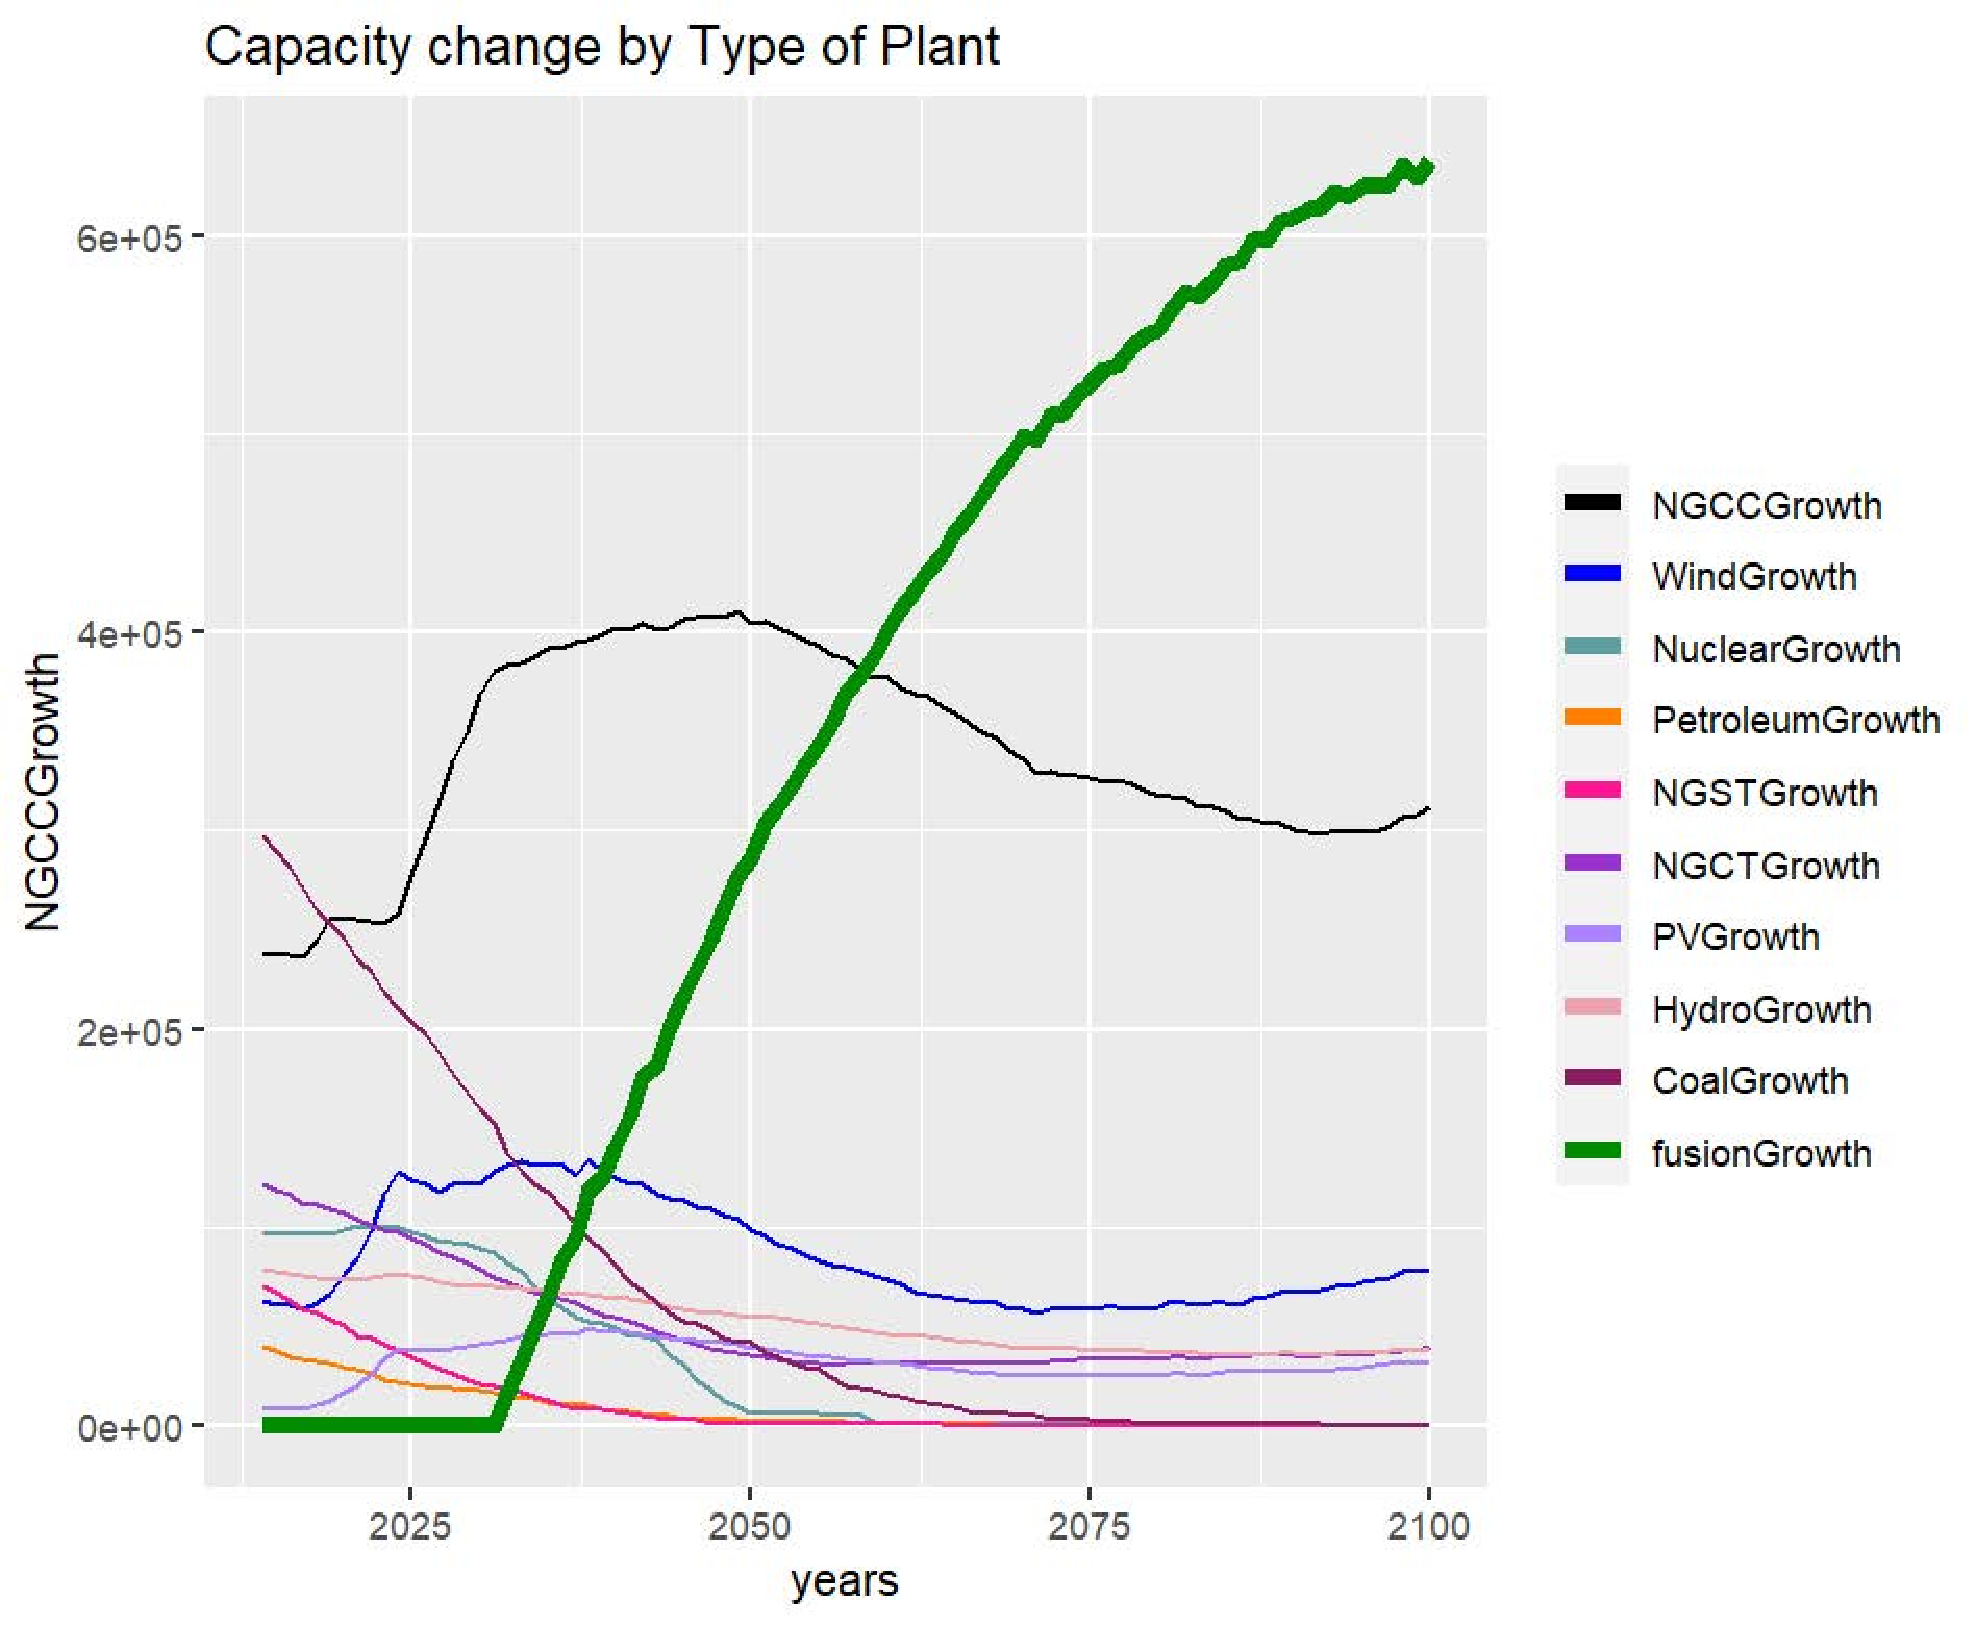
\includegraphics[width =0.65\linewidth]{SubreportFigures/spangher_default.pdf}
    \caption{'S-curve' deployment model, based on Spangher's research \cite{spangher2019characterizing}. }
    \label{fig:spangher_gdp}
\end{figure}

If MIF is perceived to stand out compared to other fusion technologies, deployment scenarios could be expected to be more optimistic, corresponding to a  faster rate of deployment in the market. 

This could, however, vary from nation to nation, and is heavily dependent on the following factors: 

Public opinion: The importance of public opinion is dependent on the regime of the region. In democratic countries, positive public opinion is essential to widespread deployment, whereas, in monarchic countries (such as Saudi Arabia), this may not be as important a factor. In Saudi Arabia, to propagate deployment, convincing members of the Saudi Royal Family would be of primary importance, with public education on  MIF being of lower priority. In the West, learning from nuclear fission, if the public perceives MIF to be dangerous, deployment is likely to be limited (e.g. Germany). The public would also have to be convinced that MIF has certain advantages over other fusion technologies and/or other energy sources.

Funding availability for R\&D: In order to be able to afford the supply chain, investments are required from public and/or private parties. This would not be possible in every country and attaining this funding would bring challenges depending on the region. 

Availabilities of a suitable workforce: scientists, engineers, technicians, etc. would be required, as well as manufacturers such as ship welders. The relative availability of required workforces will vary by region.

There are multiple other factors that play a role but these three factors are the most important limits to deployment in any deployment scenario. We can use Spanghers’ model again to model different deployment scenarios given how significant the limits to deployment are, as shown below. If the limits to deployment are significant in a particular deployment scenario (for example, there may be a lack of funding available or a public backlash), then this may slow down deployment to 10\%. If the challenges aren’t as significant, then we would see a deployment scenario closer to 80\%. 

\begin{figure}[h!]
    \centering
    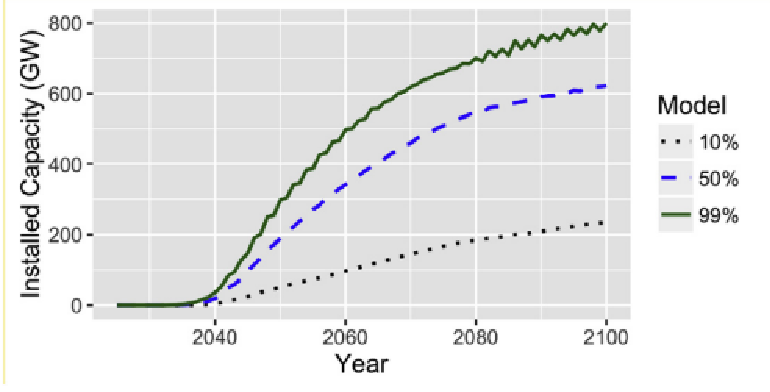
\includegraphics[width =0.65\linewidth]{SubreportFigures/spangher_limits.pdf}
    \caption{'S-curve' deployment model under various scenarios, based on Spangher's research \cite{spangher2019characterizing}. }
    \label{fig:spangher_gdp}
\end{figure}
 

\subsection{Conclusions}

In this risk assessment of Magnetic Mirror Inertial Fusion (MIF) for investors, the multifaceted nature of uncertainties and opportunities it presents is evident. The primary risks are presented by the extended timeframe, technological considerations,  macroscopic market factors, public perception, safety concerns, supply chain limits to deployment, and regional variations. Nevertheless, it is evident that fusion energy, specifically MIF, emerges as a pivotal technology in the context of the Paris Climate Agreement, with the potential to reshape the global energy sector.

MIF is approaching technological feasibility but faces uncertainties related to its long development timeline and changing technology requirements. For investors, this means facing a scenario where immediate financial returns are uncertain, but the potential long-term environmental, financial, and social benefits are significant. Studies like those of Klingelhöfer and Kurz indicate that in an energy market driven by strict environmental policies, MIF could become increasingly significant, potentially leading to reduced energy system costs and carbon taxes \cite{klingelhofer2011financial}. The IND model by Landis and Rausch also points to a favorable shift towards renewable technologies like MIF under low-carbon policies, especially due to its dispatchability in reserve markets, giving it an edge over existing renewables  \cite{landis2017deep}.

Public perception plays a critical role in the deployment of MIF. Effective and informed public engagement is necessary to overcome historical skepticism towards nuclear technologies, as highlighted by the National Nuclear Laboratory’s initiatives \cite{tol2022costs}. The successful deployment of MIF also hinges on addressing these public concerns, along with demonstrating its safety and environmental benefits.

Importantly, the notion of impact investing emerges as a significant factor. Investors are increasingly considering nonpecuniary benefits alongside financial returns, as evidenced by the findings of Barber et al. \cite{barber2021impact}. This willingness to accept lower financial returns for broader environmental and social gains is crucial in understanding the investment landscape for MIF.

In conclusion, it is clear that while fusion faces significant uncertainties - technical uncertainties, public perception issues, and complex financial viability - its potential as a sustainable and long-term energy solution is immense. For investors, the decision to invest in MIF should be guided not only by traditional financial metrics but also by the broader, nonpecuniary benefits it offers. This approach is pivotal in a world gravitating towards sustainable energy solutions, with MIF potentially playing a critical role in this transition. The risk assessment thus underscores the need for a nuanced investment approach that balances immediate financial uncertainties with long-term environmental and societal returns.